\documentclass{beamer}
\mode<presentation> {
\usetheme{Amsterdam}
\setbeamertemplate{navigation symbols}{}}
\usepackage[utf8]{inputenc}
\usepackage{graphicx}
\usepackage{booktabs}

%----------------------------------------------------------------------------------------
%	TITULOS
%----------------------------------------------------------------------------------------
\title[Seminario de tecnologia]{Unidad IV\\ Sensores}
\author{David A. Trejo Pizzo}
\institute[Instituto Multimedial Da Vinci]
{Departamento de sistemas\\
\medskip
\textit{dtrejopizzo@gmail.com}}
\date{Marzo, 2015}

\begin{document}
\begin{frame}
\titlepage
\end{frame}


%----------------------------------------------------------------------------------------
%	INDICE
%----------------------------------------------------------------------------------------
\begin{frame}
\frametitle{Estructura}
\tableofcontents
\end{frame}


%----------------------------------------------------------------------------------------
%	SLIDES
%----------------------------------------------------------------------------------------

\section{Introducción}

\begin{frame}
\frametitle{Adquisición de datos}
\begin{itemize}
\item asasa
\item asasa
\item asasa
\end{itemize}
\begin{figure}[!h]
\centering
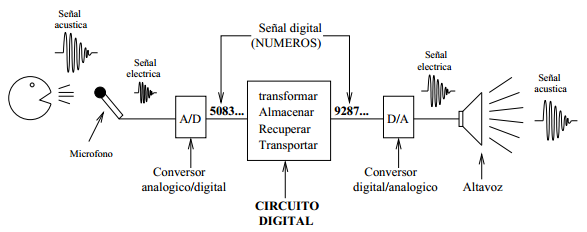
\includegraphics[width=2in]{procmuestreo}
\end{figure}
\end{frame}
%------------------------------------------------

\begin{frame}
\frametitle{Sensores}
\begin{itemize}
\item Es un dispositivo capaz de detectar magnitudes físicas o químicas, llamadas variables de instrumentación (impulsos), y transformarlas en variables eléctricas.
\end{itemize}
\begin{figure}[!h]
\centering
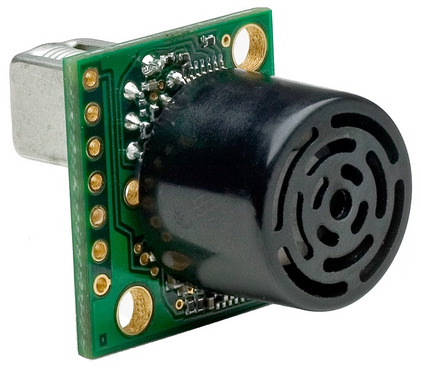
\includegraphics[width=2in]{sensor}
\end{figure}
\end{frame}
%------------------------------------------------

\subsection{Clasificación de sensores}

\begin{frame}
\frametitle{Clasificación de sensores}
\begin{itemize}
\item Propioceptivos/exteroceptivos
\begin{itemize}
\item Los sensores propioceptivos miden valores internos para el robot como por ejemplo, velocidad del motor.
\item Los sensores exteroceptivos obtienen información del entorno del robot, como la distancia a objetos.
\end{itemize}
\item Activos/Pasivos
\begin{itemize}
\item Los sensores pasivos utilizan la energía proveniente del medio ambiente (por ejemplo, la sonda de temperatura).
\item Los sensores activos emiten energía luego medir la reacción (por ejemplo sonar).
\end{itemize}
\end{itemize}
\end{frame}
%------------------------------------------------

\begin{frame}
\frametitle{Tipos de sensores}
\begin{figure}[!h]
\centering
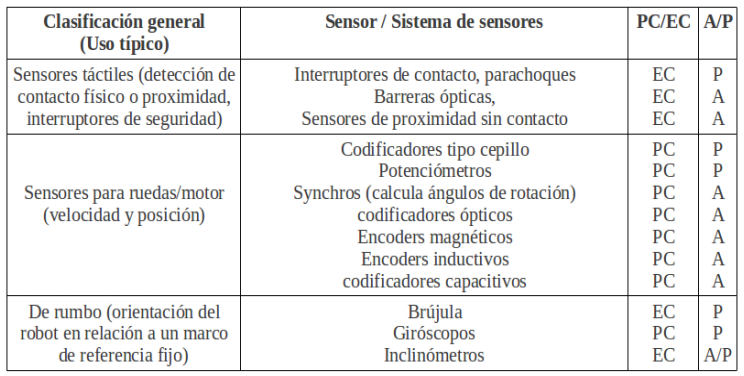
\includegraphics[width=4in]{tipo1}
\end{figure}
\end{frame}
%------------------------------------------------

\begin{frame}
\frametitle{Tipos de sensores}
\begin{figure}[!h]
\centering
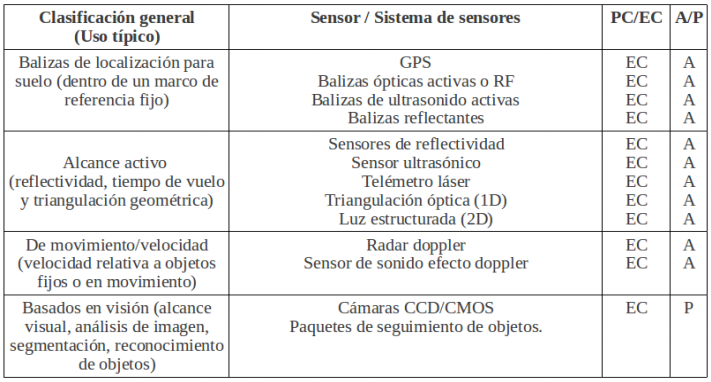
\includegraphics[width=4in]{tipo2}
\end{figure}
\end{frame}
%------------------------------------------------

\subsection{Caracteristicas}

\begin{frame}
\frametitle{Alcance y resolución}
\begin{itemize}
\item Alcance (rango)
\begin{itemize}
\item Límites inferior y superior.
\item Por ejemplo, un sensor IR mide la distancia entre 10 y 80 cm.
\end{itemize}
\item Resolución
\begin{itemize}
\item Es la mínima diferencia entre dos mediciones.
\item Para sensores digitales por lo general la resolución es la resolución A/D. Ejemplo: 5V/255 (8 bits) = 0,02 V
\end{itemize}
\end{itemize}
\end{frame}
%------------------------------------------------

\begin{frame}
\frametitle{Rango Dinámico}
\begin{itemize}
\item Es usado para medir la diferencia entre los límites inferior y superior de las entradas del sensor.
\item Formalmente, es la relación entre el máximo y el mínimo de entrada mensurable, normalmente en decibels (dB).
\item Dynamic Range = 10 log [UpperLimit / LowerLimit]
\item Por ejemplo, un sensor de sonar mide hasta una distancia máxima de 3 m, con límite inferior de 1 cm.
\item Dynamic Range = 10 log [3 / 0.01] = 24,8 dB
\end{itemize}
\end{frame}
%------------------------------------------------

\begin{frame}
\frametitle{Linealidad}
\begin{itemize}
\item Una medida de cómo la relación lineal entre la señal de salida del sensor y la señal de entrada.
\item La linealidad es menos importante cuando la señal es tratada después con una computadora.
\item Ejemplos:
\begin{itemize}
\item Considere el rango de medición de un sensor de rango IR.
\item Sea x la medida real en metros, sea y la salida del sensor en voltios, y la función y = f (x).
\end{itemize}
\begin{figure}[!h]
\centering
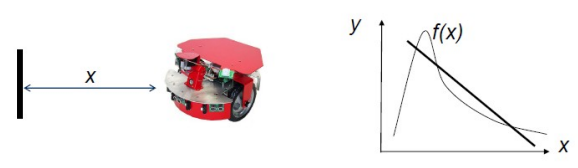
\includegraphics[width=2in]{linealidad}
\end{figure}
\end{itemize}
\end{frame}
%------------------------------------------------

\begin{frame}
\frametitle{Ancho de banda o Frecuencia}
\begin{itemize}
\item Es la velocidad con la que un sensor puede representar un flujo de lecturas.
\begin{itemize}
\item Generalmente hay un límite superior en función del sensor y la velocidad de muestreo
\item Ejemplo: un sonar toma mucho tiempo para obtener una señal de retorno.
\end{itemize}
\item Para el control autónomo, se desean frecuencias más altas.
\begin{itemize}
\item Ejemplo: si una medición de GPS se produce a 1 Hz y el vehículo autónomo utiliza esto para evitar otros vehículos que estan a 1 m. de distancia.
\end{itemize}
\end{itemize}
\end{frame}
%------------------------------------------------

\begin{frame}
\frametitle{Sensibilidad}
\begin{itemize}
\item Relación de salida cambiará a cambio de entrada. 
\begin{itemize}
\item Ejemplo: un sensor de rango aumentará la tensión de salida 0,1 V por cada cm de distancia medido.
\end{itemize}
\item La sensibilidad en sí es deseable, pero podría estar acoplado con sensibilidad a otros parámetros del entorno.
\item Sensibilidad cruzada: la sensibilidad a los parámetros ambientales que son ortogonales a los parámetros de destino.
\begin{itemize}
\item Ejemplo: algunos compases son sensibles al medio ambiente local.
\end{itemize}
\end{itemize}
\end{frame}
%------------------------------------------------

\begin{frame}
\frametitle{Exactitud y precision}
\begin{itemize}
\item Exactitud es la diferencia entre la salida del sensor y el valor verdadero (es decir, error = m - v).
\begin{itemize}
\item Exactitud = $1-|m-v|/v$ donde $m$ = valor medido y $v$ = valor real.
\end{itemize}
\item Precisión es la reproducibilidad de los resultados del sensor.
\begin{itemize}
\item Precisión = rango/varianza
\end{itemize}
\end{itemize}
\end{frame}
%------------------------------------------------

\begin{frame}
\frametitle{Errores}
\begin{itemize}
\item Error sistemático
\begin{itemize}
\item Determinístico.
\item Es causado por factores que pueden ser modelados (por ejemplo, distorsión óptica en la cámara).
\end{itemize}
\item Error aleatorio
\begin{itemize}
\item No determinístico
\item No es previsible
\item Por lo general se describe probabilísticamente
\end{itemize}
\end{itemize}
\end{frame}
%------------------------------------------------

\begin{frame}
\frametitle{Errores}
\begin{itemize}
\item Las mediciones en el mundo real cambian dinámicamente y son propensas a errores.
\begin{itemize}
\item Cambio de iluminaciones.
\item Superficies absorbentes (luz o el sonido).
\end{itemize}
\item Errores sistemáticos vs. aleatorios no están bien definidos para robots móviles.
\begin{itemize}
\item Hay una sensibilidad cruzada del sensor de robot a la pose del robot y a los cambios del medio ambiente.
\item Hay difíciles para modelar el comportamiento, parecen ser al azar.
\end{itemize}
\end{itemize}
\end{frame}
%------------------------------------------------


\subsection{Incertidumbre}

\begin{frame}
\frametitle{Representación}
\begin{itemize}
\item Describir medición como una variable aleatoria X.
\item Dado un conjunto de n mediciones con valores phi.
\item Caracterizar las propiedades estadísticas de X con una función de densidad de probabilidad f(x).
\end{itemize}
\begin{figure}[!h]
\centering
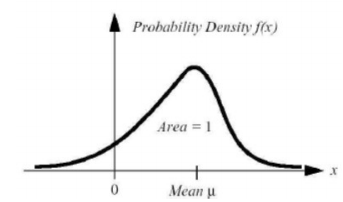
\includegraphics[width=2in]{distri}
\end{figure}
\end{frame}
%------------------------------------------------

\begin{frame}
\frametitle{Probabilidades}
El valor esperado de X es la media
$$\mu = E[X] = \int_{-\infty}^{\infty} xf(x) dx$$
La varianza de X es
$$\sigma^{2}= var(x) = \int_{-\infty}^{\infty} (x-\mu)^{2} xf(x) dx$$
\end{frame}
%------------------------------------------------

\section{Sensores}

\begin{frame}
\frametitle{Encoders}
\begin{itemize}
\item Un codificador óptico digital es un dispositivo que convierte el movimiento en una secuencia de pulsos digitales. Al contar un solo bit o mediante la descodificación de un conjunto de bits, los pulsos se pueden convertir en mediciones de la posición relativa o absoluta.
\item Codificadores ópticos son sensores propioceptivos.
\item Se puede integrar la señal para obtener la posición del robot.
\item Dos tipos principales:
\begin{itemize}
\item Codificadores absolutos: miden la orientación actual de la rueda.
\item Codificadores incrementales: miden el cambio en la orientación de una rueda.
\end{itemize}
\end{itemize}
\end{frame}
%------------------------------------------------

\begin{frame}
\frametitle{Sensores de rango}
Los sensores de rango hacen uso de la velocidad de propagación de ondas sonoras o electromagnéticas respectivamente.\\

La distancia recorrida por una onda esta dada por: $d = c*t$
\begin{itemize}
\item d = distancia recorrida
\item c = velocidad de propagación de las ondas
\item t = tiempo
\end{itemize}
\end{frame}
%------------------------------------------------

\begin{frame}
\frametitle{Sensores de rango}
\begin{itemize}
\item Para sonido: v = 0.3 m/ms
\item Para ondas electromagneticas: v = 0.3 m/ns
\end{itemize}

Si la distancia fuera de 3 metros, entonces

\begin{itemize}
\item $t_{ultrasonic}$ = 10 ms
\item $t_{laser}$ = 10 ns (laser es dificil de medir, además son caros)
\end{itemize}
\end{frame}
%------------------------------------------------

\begin{frame}
\frametitle{Sensores de rango - Calidad}
La calidad de los sensores de rango dependerá de:\\
\begin{itemize}
\item Las incertidumbres del tiempo de llegada de la señal reflejada.
\item Las imprecisiones en el tiempo de medida de vuelo (láser).
\item Ángulo de haz transmitido (sonido).
\item Interacción con el objetivo (reflexiones especulares).
\item Variación de la velocidad de propagación.
\end{itemize}
\end{frame}
%------------------------------------------------

\begin{frame}
\frametitle{Sensores de rango - Ultrasonido}
\begin{itemize}
\item El sensor transmite un paquete de ondas de presión por ultrasonido $d = c t / 2$
\item La velocidad del sonido c es 340 m/s en el aire
\begin{itemize}
\item $c = \sqrt{\gamma RT}$
\item $\gamma$ es la relación de calores específicos.
\item R = constante de los gases.
\item T = temperatura en grados Kelvin.
\end{itemize}
\end{itemize}
\end{frame}
%------------------------------------------------

\begin{frame}
\frametitle{Sensores de rango - Ultrasonido}
\begin{columns}[c]
\column{.5\textwidth}
\begin{itemize}
\item Frecuencia típicamente 40 - 180 kHz
\item La onda generada por el transductor piezoeléctrico.
\item El receptor puede coincidir con el transmisor (Problema con objetos muy cercanos, tiempo ciego).
\item El haz de sonido no se propaga en el cono, sino en puntos.
\end{itemize}
\column{.5\textwidth}
\begin{figure}[!h]
\centering
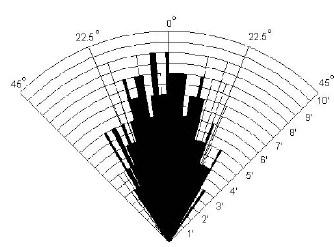
\includegraphics[width=2in]{ultrasonido}
\end{figure}
\end{columns}
\end{frame}
%------------------------------------------------

\begin{frame}
\frametitle{Detectores de rumbo}
\begin{itemize}
\item Se puede determinar la orientación y la inclinación del robot.
\item Pueden ser propioceptivos (giroscopio, por ejemplo) o exteroceptivos (brújula, por ejemplo).
\item Se utilizan junto a la información de velocidad de los codificadores para obtener una estimación de la posición del robot.
\end{itemize}
\end{frame}
%------------------------------------------------

\begin{frame}
\frametitle{El compas}
\begin{itemize}
\item Más de 4000 años de antigüedad.
\item Utiliza el campo magnético de la Tierra para proporcionar medida absoluta para la orientación.
\item Desventajas: el campo magnético de la Tierra es débil. El campo es fácilmente perturbado por otros  objetos magnéticos.
\item No es confiable para ambientes interiores.
\end{itemize}
\end{frame}
%------------------------------------------------

\subsection{Sistema de balizas terrestres}

\begin{frame}
\frametitle{Sistema de balizas terrestres}
\begin{itemize}
\item Se utiliza para la localización.
\item Utilizado por los seres humanos (por ejemplo, las estrellas, los faros).
\item Las balizas pueden ser activas o pasivas.
\item Conociendo la ubicación de las balizas se puede realizar la localización.
\item El problema es que no son flexibles.
\end{itemize}
\begin{figure}[!h]
\centering
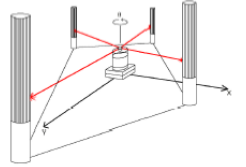
\includegraphics[width=2in]{Balizas}
\end{figure}
\end{frame}
%------------------------------------------------

\begin{frame}
\frametitle{Auto calibración PseudoLite K9}
\begin{figure}[!h]
\centering
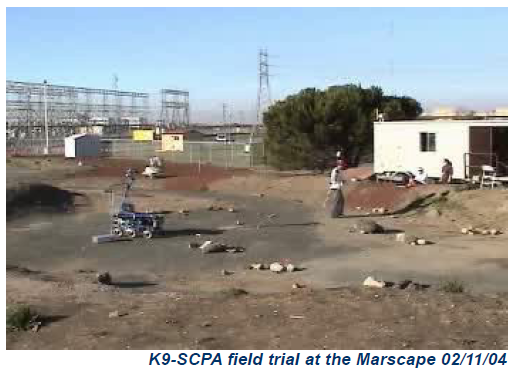
\includegraphics[width=3in]{Self}
\end{figure}
\end{frame}
%------------------------------------------------

\subsection{Vision}

\begin{frame}
\frametitle{Sistemas de visión}
\begin{itemize}
\item La visión es nuestro sentido más poderoso porque nos proporciona una enorme cantidad de información sobre el medio ambiente, sin tener contacto directo.
\item Se aplica mucho esfuerzo en equipar máquinas con visión.
\end{itemize}
\begin{figure}[!h]
\centering
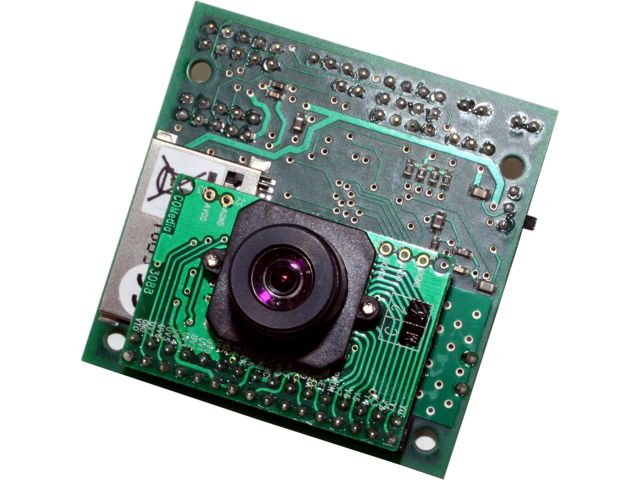
\includegraphics[width=2in]{cam1}
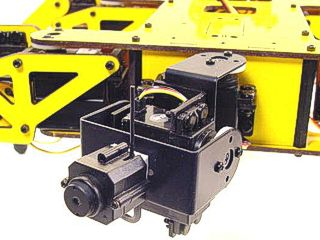
\includegraphics[width=2in]{cam2}
\end{figure}
\end{frame}
%------------------------------------------------

\begin{frame}
\frametitle{Sistemas de visión}
\begin{itemize}
\item La visión es también nuestro sentido más complicado. Si bien podemos reconstruir puntos de vista con alta resolución en papel, la comprensión de cómo el cerebro procesa la información todavía no esta muy desarrollada.
\item Sensores de alcance visual en estéreo.
\item El movimiento y el flujo óptico.
\item Sensores de seguimiento por color.
\end{itemize}
\end{frame}
%------------------------------------------------

\begin{frame}
\frametitle{Visión Monocular}
\begin{itemize}
\item Problema con visión monocular es que no se puede saber hasta qué punto algo es del robot. No 
Distancia de la información!
\item Observa la siguiente imagen de una pelota de color rojo:
\begin{figure}[!h]
\centering
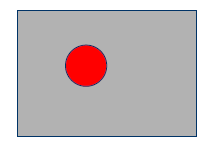
\includegraphics[width=1in]{vision1}
\end{figure}
\item Dependiendo del tamaño de la bola, podría estar situada más cerca (posición 2) o más (posición 1) de 
la cámara
\end{itemize}
\end{frame}
%------------------------------------------------

\begin{frame}
\frametitle{Visión estéreo}
\begin{itemize}
\item El uso de dos cámaras proporciona información suficiente para darnos la gama a la pelota.
\item La intersección de los dos conos debe ser donde la pelota descansa.
\begin{figure}[!h]
\centering
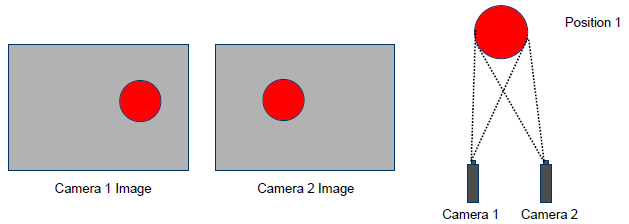
\includegraphics[width=3in]{vision2}
\end{figure}
\end{itemize}
\end{frame}
%------------------------------------------------

\begin{frame}
\frametitle{Visión estéreo}
\begin{itemize}
\item Considere la posibilidad de geometría idealizada cámara.
\item Comparar proyección de una diana en 2 planos de imagen.
\end{itemize}
\begin{figure}[!h]
\centering
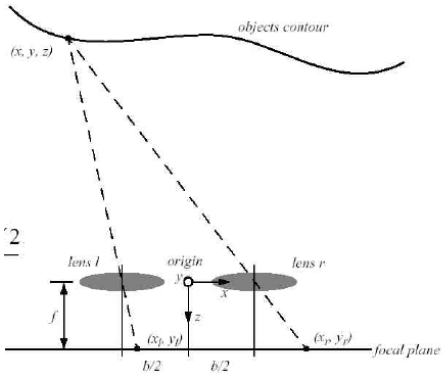
\includegraphics[width=2in]{stereo0}
\end{figure}
\end{frame}
%------------------------------------------------

\begin{frame}
\frametitle{Laser}
\begin{itemize}
\item Rayos transmitidos y recibidos coaxiales.
\item El transmisor se ilumina con un haz blanco.
\item El receptor detecta el tiempo necesario para ida y vuelta.
\item Se puede obtener información 2D y 3D utilizando barridos en espejo
\end{itemize}
\begin{figure}[!h]
\centering
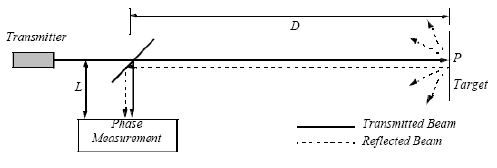
\includegraphics[width=2in]{laser1}
\end{figure}
\end{frame}
%------------------------------------------------

\section{GPS}

\begin{frame}
\frametitle{Global Positioning System (GPS)}
\begin{figure}[!h]
\centering
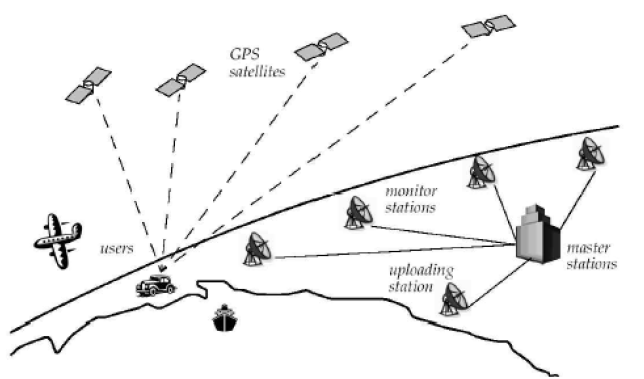
\includegraphics[width=3in]{GPS}
\end{figure}
\end{frame}
%------------------------------------------------

\begin{frame}
\frametitle{Global Positioning System (GPS)}
\begin{itemize}
\item Desarrollado para uso militar.
\item Ahora accesible para uso comercial (por ejemplo, senderismo, vuelo, etc.).
\item Hay 24 satélites que orbitan la Tierra cada 12 horas a la altura del +20 km.
\item Hay 4 satélites situados en cada uno de 6 planos inclinados a 55 grados respecto al Ecuador.
\end{itemize}
\end{frame}
%------------------------------------------------

\begin{frame}
\frametitle{Global Positioning System (GPS)}
\begin{itemize}
\item Se utiliza un receptor GPS para medir el tiempo de vuelo de varios satélites al receptor. El sistema requiere:
\begin{itemize}
\item Tiempo de sincronización entre satélites y el receptor. (relatividad, dilatación temporal).
\item Conocida la posición de los satélites.
\item La medición precisa del tiempo de vuelo.
\item La superación de la interferencia con otras señales.
\end{itemize}
\end{itemize}
\end{frame}
%------------------------------------------------

\begin{frame}
\frametitle{Global Positioning System (GPS)}
\begin{itemize}
\item Sincronización de la hora:
\begin{itemize}
\item Los relojes atómicos de cada satélite se controlan desde las estaciones terrestres.
\end{itemize}
\item Ubicación conocida de los satélites:
\begin{itemize}
\item Una serie de estaciones terrestres ampliamente distribuidas controlan los satélites.
\item Un análisis de las mediciones de la estación maestra y la posición de cada satélite se transmite a las estaciones de base. 
\end{itemize}
\end{itemize}
\end{frame}
%------------------------------------------------

\begin{frame}
\frametitle{Global Positioning System (GPS)}
\begin{itemize}
\item Medición precisa:
\begin{itemize}
\item Satélites transmiten (al mismo tiempo) el tiempo actual y la ubicación.
\item Las diferencias de hora de llegada informar al receptor de la distancia relativa a cada satélite.
\item Se necesita de cuatro satélites para resolver por (x, y, z) y la corrección T de reloj
\end{itemize}
\item Los sensores GPS regulares y de buena calidad, pueden obtener una precisión de 10-15 metros.
\item Con un segundo receptor de posición conocida, el GPS diferencial (DGPS) se puede corregir el error hasta 1 metro.
\item Fase de portador puede obtener resolución DGPS hasta 1 centimetro (solo en aplicaciones de defensa).
\end{itemize}
\end{frame}
%------------------------------------------------

\begin{frame}
\frametitle{Global Positioning System (GPS)}
\begin{figure}[!h]
\centering
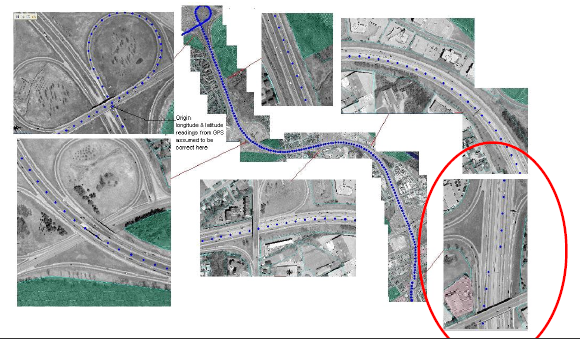
\includegraphics[width=3in]{GPS2}
\end{figure}
\end{frame}
%------------------------------------------------

\section{Wireless Sensor Networks}

\begin{frame}
\frametitle{Redes de sensores inhalambricos}
\begin{itemize}
\item A pesar de que los sensores inalámbricos ha limitado los recursos en la memoria, potencia de cálculo, el ancho de banda, y la energía.
\item Con un tamaño pequeño. Puede ser integrado en el entorno físico.
\item Soporte potente servicio en forma agregada (interacción / colaboración entre los nodos).
\item Multi-hop redes ad-doc de auto-organización.
\item Computación ubicua / sensorización.
\end{itemize}
\end{frame}
%------------------------------------------------

\begin{frame}
\frametitle{Redes de sensores inhalambricos}
\begin{itemize}
\item Consisten en grupos de dispositivos que utilizan tecnologías de sensores desplegados en un área específica.
\item Se comunican datos de manera inalámbrica a un sistema central. 
\item Las redes de sensores supervisan continuamente los procesos químicos, físicos o propiedades magnéticas, utilizando la infraestructura de comunicaciones existente.
\end{itemize}
\end{frame}
%------------------------------------------------

\begin{frame}
\frametitle{Nodos (motes)}
\begin{itemize}
\item Se compone de muchos nodos sensores minúsculos, cada una equipada con un transceptor de radio, un microprocesador y un número de sensores.
\item Cada nodo tiene una capacidad de procesamiento autónoma, los datos pueden ser procesados a medida que pasan a través de la red. 
\item Dadas las limitaciones de los equipos y el entorno físico y niveles de alta demanda con la que los nodos deben operar, algoritmos y protocolos deben ser diseñados para proporcionar el consumo de energía fuerte y eficiente.
\end{itemize}
\end{frame}
%------------------------------------------------

\subsection{Topologias}

\begin{frame}
\frametitle{Topologias}
\begin{itemize}
\item Estrella: todos los nodos conectados a un punto de enlace.
\item Arbol: nodos conectados a routers, a su vez conectados en un gateway central.
\item Red: nodos conectados a routers, a su vez interconectados entre si y terminados en un gateway central.
\end{itemize}
\frametitle{Topologias}
\begin{figure}[!h]
\centering
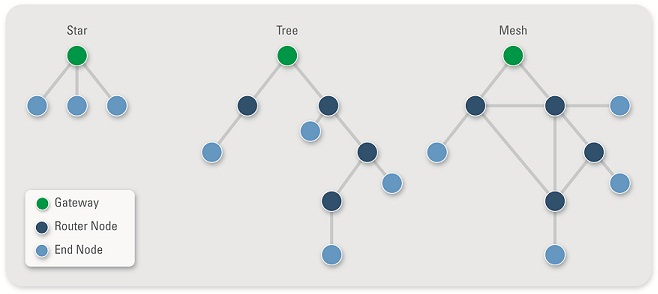
\includegraphics[width=2.5in]{topologias}
\end{figure}
\end{frame}
%------------------------------------------------

\begin{frame}
\frametitle{Redes mesh}
\begin{itemize}
\item Permiten que los datos "salten" de un nodo a otro. Cada nodo es capaz de comunicarse entre sí, generando multiples rutas o "paths".
\end{itemize}
\begin{figure}[!h]
\centering
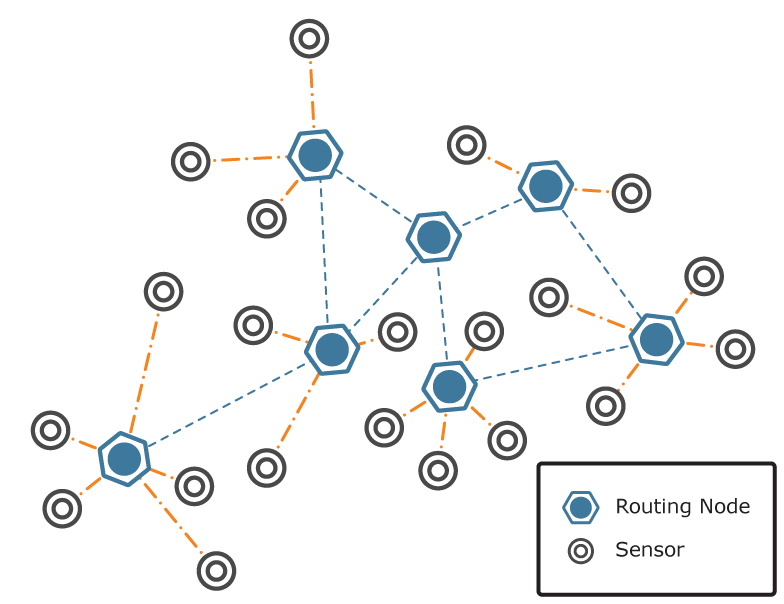
\includegraphics[width=2.5in]{wsn}
\end{figure}
\end{frame}
%------------------------------------------------

\begin{frame}
\frametitle{asas}
\begin{itemize}
\item 
\item 
\item 
\end{itemize}
\begin{figure}[!h]
\centering
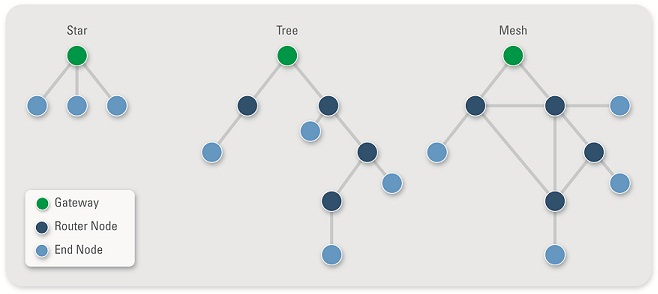
\includegraphics[width=2.5in]{topologias}
\end{figure}
\end{frame}
%------------------------------------------------

\subsection{Protocolos}

\begin{frame}
\frametitle{a}
\begin{itemize}
\item 
\item 
\item 
\end{itemize}
\begin{figure}[!h]
\centering
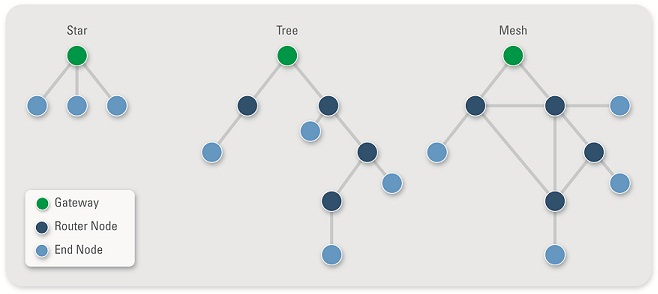
\includegraphics[width=2.5in]{topologias}
\end{figure}
\end{frame}
%------------------------------------------------

\begin{frame}
\frametitle{a}
\begin{itemize}
\item 
\item 
\item 
\end{itemize}
\begin{figure}[!h]
\centering
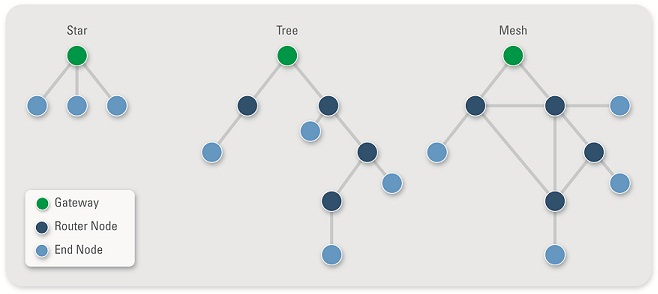
\includegraphics[width=2.5in]{topologias}
\end{figure}
\end{frame}
%------------------------------------------------

\begin{frame}
\frametitle{asas}
\begin{itemize}
\item 
\item 
\item 
\end{itemize}
\begin{figure}[!h]
\centering
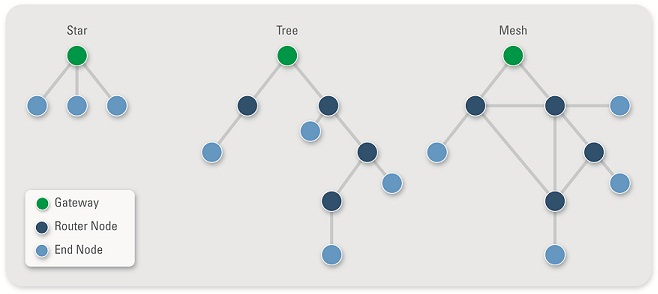
\includegraphics[width=2.5in]{topologias}
\end{figure}
\end{frame}
%------------------------------------------------

\begin{frame}
\frametitle{asas}
\begin{itemize}
\item 
\item 
\item 
\end{itemize}
\begin{figure}[!h]
\centering
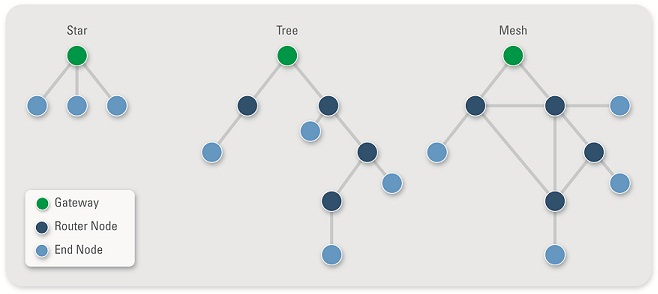
\includegraphics[width=2.5in]{topologias}
\end{figure}
\end{frame}
%------------------------------------------------

\begin{frame}
\frametitle{asas}
\begin{itemize}
\item 
\item 
\item 
\end{itemize}
\begin{figure}[!h]
\centering
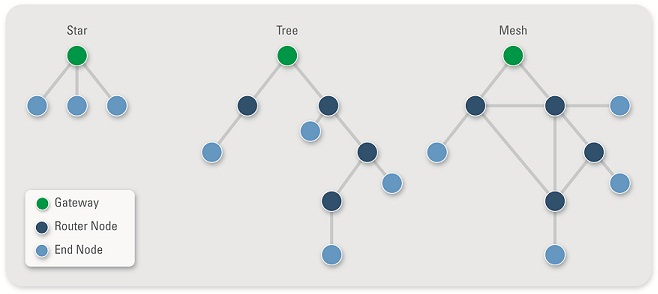
\includegraphics[width=2.5in]{topologias}
\end{figure}
\end{frame}
%------------------------------------------------

\subsection{Aplicaciones}

\begin{frame}
\frametitle{Agricultura}
\begin{itemize}
\item 
\item 
\item 
\end{itemize}
\begin{figure}[!h]
\centering
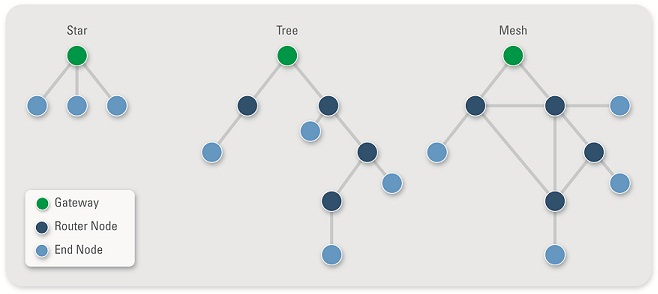
\includegraphics[width=2.5in]{topologias}
\end{figure}
\end{frame}
%------------------------------------------------

\begin{frame}
\frametitle{Control de plagas}
\begin{itemize}
\item 
\item 
\item 
\end{itemize}
\begin{figure}[!h]
\centering
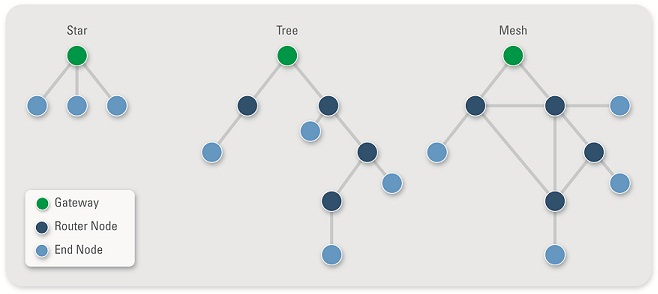
\includegraphics[width=2.5in]{topologias}
\end{figure}
\end{frame}
%------------------------------------------------

\begin{frame}
\frametitle{Interaccion entre personas}
\begin{itemize}
\item 
\item 
\item 
\end{itemize}
\begin{figure}[!h]
\centering
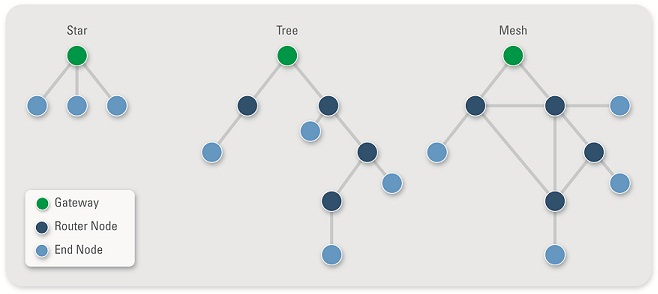
\includegraphics[width=2.5in]{topologias}
\end{figure}
\end{frame}
%------------------------------------------------

\begin{frame}
\frametitle{Trafico inteligente}
\begin{itemize}
\item 
\item 
\item 
\end{itemize}
\begin{figure}[!h]
\centering
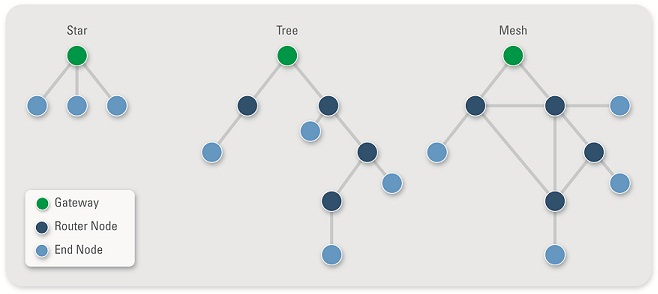
\includegraphics[width=2.5in]{topologias}
\end{figure}
\end{frame}
%------------------------------------------------

\end{document}